\section{Implementation}\label{sec:Implementation}
% ! Nuclear option: Linux dual-boot and screenshot as you go on it.

\subsection{Software requirements}
% Talk about Visual Studio Code.
% Talk about Python and the modules themselves. Did any of them have logins?
% Talk about OpenAI setup.
The project was developed using Visual Studio Code as a development environment and Python as the programming language.
Both of these are available freely with no limitation for academic use.

\para Many Python modules were used, with the UV package manager \autocite{astralUv} being used for their installation 
due to its own high speed and ease of use. The version of Python used was 3.10.16 to ensure compatibility with the wide variety 
of modules used, which are detailed in Table \ref{tab:PythonModules}.

\begin{longtable}{ | p{0.25\textwidth} | p{0.7\textwidth} | }
    \hline
    \cellcolor{blue!25} Module(s) & \cellcolor{blue!25} Purpose \\
    \hline
    langchain & The framework used to handle LLM interactions, as well as embedding documents and user queries. \\
    \hline
    langchain-community & Provides additional helper classes and functions to assist development. \\
    \hline 
    langchain-openai \newline 
    openai & Provides the functions used to interact with OpenAI models such as gpt-4o-mini and text-embedding-3-small in LangChain. \\
    \hline 
    langgraph & Used to create a directed sequence of events for the chatbot to execute. A major part of the backend, further described 
    in Section \ref{sec:ChatbotBackend}. \\
    \hline
    pdfminer-six \newline 
    pypdf & Dependencies of LangChain for PDF reading. \\
    \hline 
    Streamlit & Used as the frontend of the chatbot and also stores the conversation in memory. Described further in Section 
    \ref{sec:ChatbotFrontend}. \\
    \hline
    \caption{The Python modules used in the project's development.}\label{tab:PythonModules}
\end{longtable}



\subsection{Data storage}
% Talk about getting University policies from their site. Provide URL or Harvard reference it?
% Talk about your own added info document you made in LaTeX.
% Talk about embedding the policies.
The backbone of this project is the BCU-related data that the chatbot will pull from when queried.
The vast majority of this data was sourced from the official Birmingham City University website \autocite{bcuPoliciesProcedures},
where individual policies are stored as PDF files for public download without any access limitations or restrictions.
An observation made through an analysis of many of the policies was that none of them explicitly state key information about the university,
such as campus building locations or information about its student union. Therefore, an additional document of my own creation with \LaTeX
was included amongst the downloaded data. This document contained key information about BCU itself, with information on campus addresses 
and miscellaneous helpful information for students.

\para With all documents downloaded or created, the next stage would be to incorporate them in a format an LLM can interpret. This introduces 
LangChain, a popular framework for LLM app development \autocite{langchain_introduction_nodate}, which provides helper classes to directly read 
PDF files from a directory and split the text data within into smaller chunks, as seen in Figure \ref{fig:LangChainDocumentLoader}.

\begin{figure}[H]
    \centering
    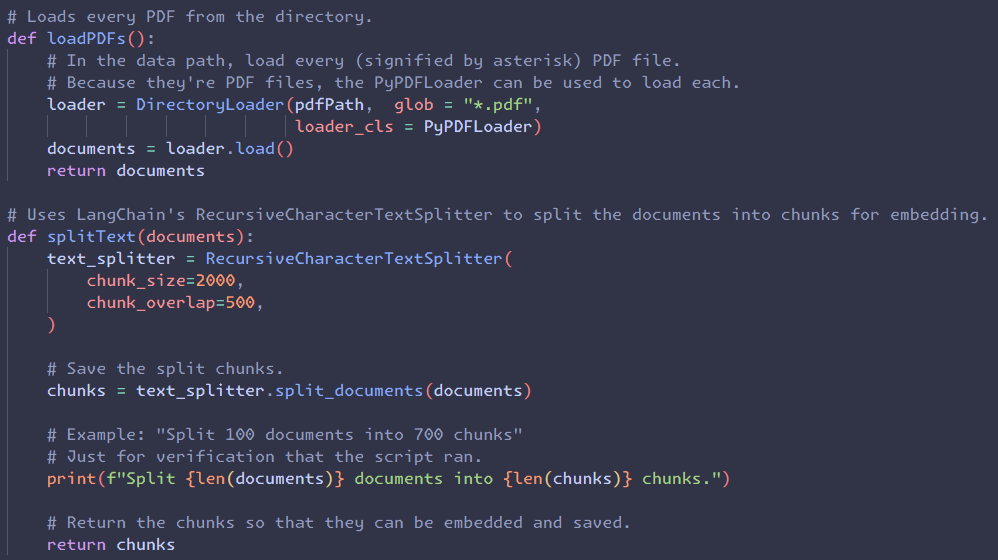
\includegraphics[width=0.8\textwidth]{Artefact/DocumentLoader.png}
    \caption{Code used to load all PDFs from the Policies directory and split them into chunks. \label{fig:LangChainDocumentLoader}}
\end{figure}

\noindent Multiple chunk sizes and overlaps were tested during the artefact's development, with an eventual settlement on 2000 character 
chunks with 500 character overlaps being used. Maximising the size of chunks is a key part in assisting the chatbot's retrieval process,
as it will be able to fetch more data with a single query which allows it to answer questions with greater detail and factual accuracy.
The chunk overlap defines how many characters appear across multiple sequential chunks, ensuring that key information is unlikely to be 
split over multiple chunks where the chatbot then may be unable to cite it. LangChain's RecursiveCharacterTextSplitter also provides 
additional arguments for a custom length function if desired, though there was no need in this project, as well as adding start indexes 
to each vector, which adds metadata stating the numerical ID of each chunk as determined by the sequential order they are split in. 

\para Once these chunks have been created, they must then be embedded as vectors, which will allow an LLM to interpret them. These 
vectors were then stored in a Facebook AI Similarity Search (FAISS) database as researched in Section \ref{sec:LitReviewRAG}, which 
ensured that the policies only needed to be embedded once rather than every time the chatbot was run, and would be retrieved 
at high speeds thanks to FAISS' efficiency.

\begin{figure}[H]
    \centering
    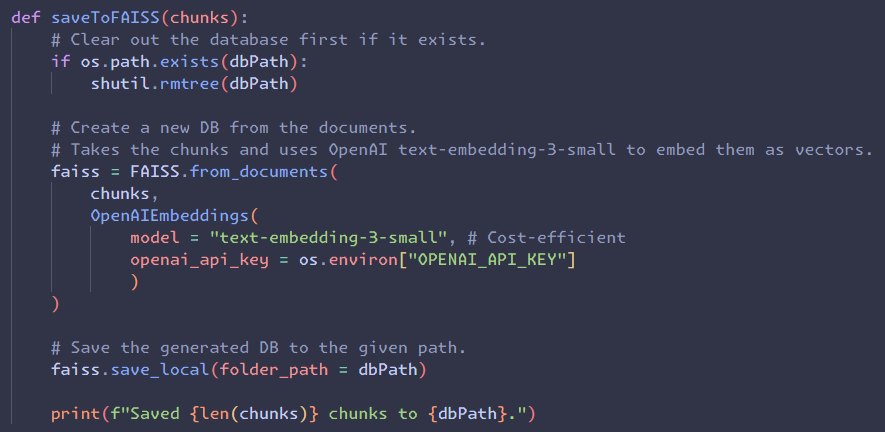
\includegraphics[width=0.8\textwidth]{Artefact/SaveToFAISS.png}
    \caption{Code used to embed and store the chunks into a FAISS DB. \label{fig:LangChainStoreFAISS}}
\end{figure}

\noindent Firstly, any existing database in the specified directory is cleared to ensure that there are no I/O errors when attempting 
to save to the directory. LangChain provides wrapper functions for both the embedding and storage of this data, making it a smooth 
and simple process in very few lines of code. 

\para  The embedding model used is OpenAI's text-embedding-3-small model \autocite{openai_vector_nodate}. The motivation behind the use of this model was primarily due to its cost efficiency, with OpenAI approximating 62,500 pages can be embedded for each dollar spent. For each 
2000-character chunk, the embedding model translates it into vector space for the LLM's interpretation. The vectors are produced based on the 
semantic similarities of each word as previously discussed and visualised in Section \ref{sec:LitReviewNLP}. 

% ! Screenshot of this running if possible.



\subsection{Chatbot backend}\label{sec:ChatbotBackend}
% Talk about LangChain and LangGraph.
As previously mentioned, the core functionality of the chatbot was developed using the LangChain and LangGraph frameworks. LangChain in particular
simplifies the development process by providing various functions and classes for quick and easy integration with necessary services such 
as FAISS and the OpenAI API, with LangGraph defining the chatbot's structure as depicted in Figure \ref{fig:ChatbotLangGraph}. 

\begin{figure}[H]
    \centering
    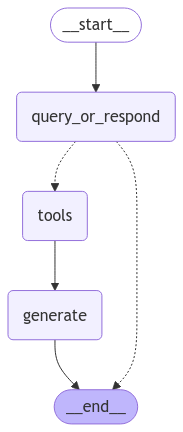
\includegraphics[width=0.3\textwidth]{Artefact/LangGraph.png}
    \caption{The graph for the chatbot. \label{fig:ChatbotLangGraph}}
\end{figure}


\para Before detailing each node of the graph, it is first necessary to establish some prerequisite variables such as the LLM itself. 
The LLM used is OpenAI's gpt-4o-mini due to cost-efficiency. The difference in performance between 4o-mini and 4o was deemed not significant 
enough for the price increase of 1500\% per 1 million tokens in relation to 4o-mini \autocite{openaiPricing}, especially considering that 4o-mini
performs suitably for the task at hand.

\para Figure \ref{fig:PrelimVariables} shows each of the variables being established, including the LLM, 
via LangChain's 'init\_chat\_model' function. The LLM is initialised with a temperature of 0, which means that it should give the same 
answer to the same prompt whenever it is given. As mentioned, this does reduce the 'personality' of the chatbot, though it greatly helps 
to reduce the potential for hallucinations in a Q\&A RAG scenario such as this one.

\begin{figure}[H]
    \centering
    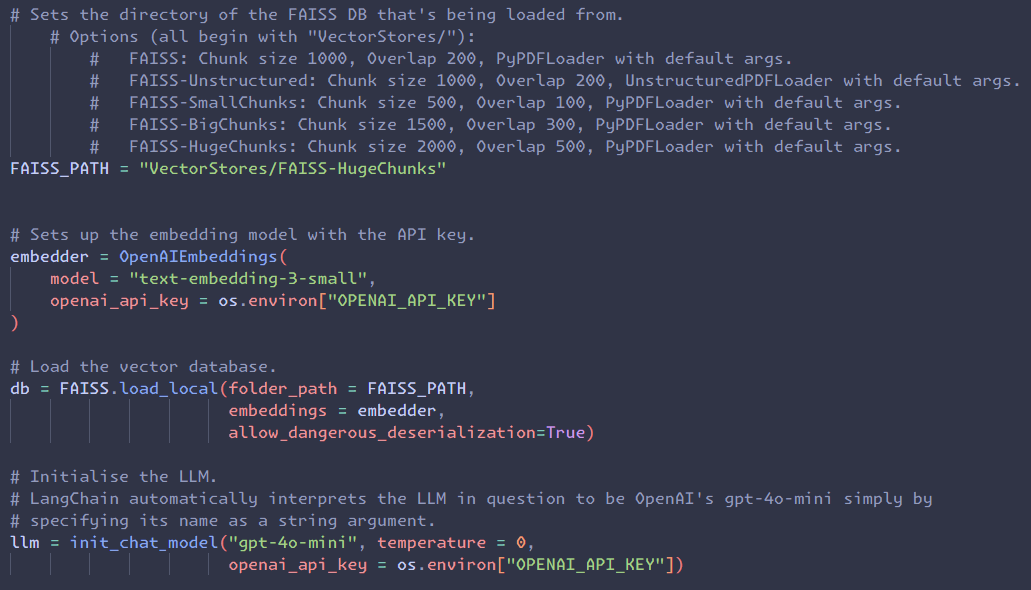
\includegraphics[width=\textwidth]{Artefact/PrelimVariables.png}
    \caption{Establishing prerequisite variables for the chatbot. \label{fig:PrelimVariables}}
\end{figure}

\noindent Thorough experimentation with the chunk sizes previously discussed in Figure \ref{fig:LangChainDocumentLoader} occurred during 
development, with the eventual decision of settling on the 2000-character chunks being made due to its more reliable performance on a set 
of sample questions discussed in Chapter \ref{ch:Evaluation}. Following the relative directory of the FAISS database being set, the 
% ! Change "chapter" to the specific relevant section when it's written.
OpenAI embedding model is once again used so that similarity searches may be performed on the database. An additional argument,
'allow\_dangerous\_deserialization', is given when loading the database. When a FAISS database is saved using LangChain, it is saved as a 
serialized file known as a Pickle file, using a .pkl file extension. It is possible for malicious code to be embedded inside these files
which could be executed when they are deserialized. However, as the files were generated specifically for this project and their contents 
are already known, it is safe to deserialize them.

\para With the prerequisite variables established, the first node of the graph was created. This is the core functionality of the LangGraph 
module, which builds on LangChain by defining an app's workflow 
as nodes and edges on a graph \autocite{langgraphLangGraph}. In development, these nodes and edges can be created, with support for conditional 
edges that ensure certain nodes such as tool calls only activate when necessary. This allows for the creation of self-directed agents which make 
decisions independently, with this functionality being used in the chatbot to decide whether a response needs BCU-related context or not. This 
occurs in the first node and entry point of the graph: the 'query\_or\_respond' node.

\begin{figure}[H]
    \centering
    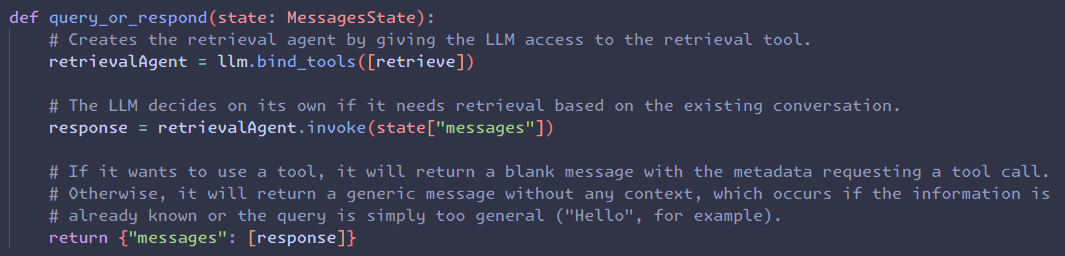
\includegraphics[width=\textwidth]{Artefact/QueryOrRespond.png}
    \caption{Code used for the 'query\_or\_respond' graph node. \label{fig:QueryOrRespond}}
\end{figure}

\noindent This function clearly demonstrates LangChain's abstractions of the backend functionality; these three lines of code
serve as the entire decision-making logic for this node, as the LLM itself will decide whether it can immediately answer the user's query,
such as in a scenario where the information they are requesting is already known from earlier in the conversation, or if their query is too 
general such as stating their name. If the LLM decides it cannot answer the query with the information it currently has available within 
the conversation, it will instead invoke the left conditional branch of the graph in Figure \ref{fig:ChatbotLangGraph} by calling on the 
retriever tool.


\subsection{Accessing the chatbot}\label{sec:ChatbotFrontend}
% Talk about Streamlit.
% Show example conversations here or perhaps make another section for them.

